\documentclass{standalone}
\usepackage{tikz}
\usepackage{pgfplots}
\pgfplotsset{compat=newest}
\usepackage{amsmath}
\usepackage[american]{circuitikz}
\usepackage{cmbright}

\definecolor{myred}{RGB}{170,0,0}
\definecolor{myblue}{RGB}{0,0,220}
\definecolor{mygreen}{RGB}{0,150,0}
\definecolor{myorange}{RGB}{255,127,0}
\definecolor{mybrown}{RGB}{150,75,0}

\begin{document}
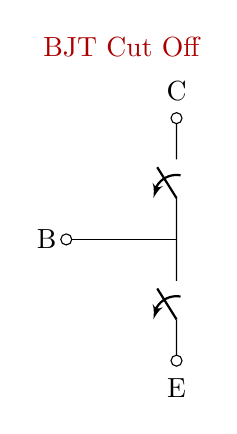
\begin{tikzpicture}
    \begin{scope}[scale=0.7]
        % Title
        \node[anchor=center, color=myred] at (1.0, 5) {BJT Cut Off};% Double diode model
        \draw (2, -0.7) to[ospst] ++(0, 2.2);
        \node[ocirc, scale=1.25] (D1E) at (2, -0.7) {};
        \node [anchor=north, color=black] at (2, -0.84) {E};
        % \draw (2, 1.5) to ++(0, 0.7) to[open] ++(0, 0.8) to ++(0, 0.7);
        \draw (2, 1.5) to[ospst] ++(0, 2.2);
        \node[ocirc, scale=1.25] (D1E) at (2, 3.7) {};
        \draw (0, 1.5) -- (2, 1.5);
        \node[ocirc, scale=1.25] (D1E) at (0, 1.5) {};
        \node [anchor=south, color=black] at (2, 3.84) {C};
        \node [anchor=east, color=black] at (0, 1.5) {B};
    \end{scope}
\end{tikzpicture}
\end{document}